%!TEX root = ../article.tex

%%%%%%%%%%%%%%%%%%%%%%%%%%%%%%%%%%%%%%%%%%%%%%%%%%%%%%%%%%%%%%%%%%%%%%%%%%%%%%%
%%%%%%%%%%%%%%%%%%%%%%%%%%%%%%%%%%%%%%%%%%%%%%%%%%%%%%%%%%%%%%%%%%%%%%%%%%%%%%%
\section{Introduction}
\label{sec:introduction}
%%%%%%%%%%%%%%%%%%%%%%%%%%%%%%%%%%%%%%%%%%%%%%%%%%%%%%%%%%%%%%%%%%%%%%%%%%%%%%%
%%%%%%%%%%%%%%%%%%%%%%%%%%%%%%%%%%%%%%%%%%%%%%%%%%%%%%%%%%%%%%%%%%%%%%%%%%%%%%%

% Let us remind first the famous Pythagoras' theorem:

% \begin{align}\label{eq:pythagore}
% 	\norm{x+y}^2 = \norm{x}^2 + \norm{y}^2 \enspace.
% \end{align}

% Note that \Cref{eq:pythagore} is ok only under some conditions.
% In terms of visualisation, you can reference a figure easily using the command \Cref{fig:pythagore} or using Fig.~\ref{fig:pythagore}.

% \begin{figure}[h] % h stands for here
% 	\centering
% 	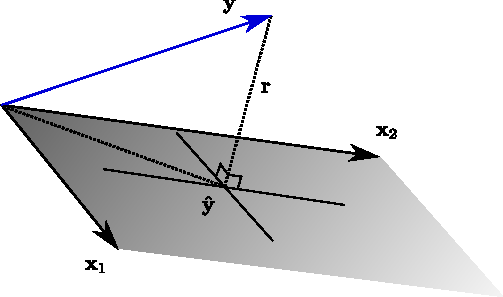
\includegraphics[width=0.6\textwidth]{residu_orth}
% 	\caption{Illustration of the residual orthogonality in least-squares.}
% 	\label{fig:pythagore}
% \end{figure}


% Also an image that is in the \texttt{prebuiltimages/} directory can also be loaded the same way:

% \begin{figure}[h] % h stands for here, ! forces even more...
% 	\centering
% 	
\includegraphics[width=0.2\textwidth]{umontpellier_logo}
% 	\caption{Illustration of a prebuiltimage available.}
% 	\label{fig:umontpellier_logo}
% \end{figure}


% For displaying side by side some images one should consider the package \lstinline+subcaptions+, that can be loaded with the \LaTeX command:

% \begin{lstlisting}[language=tex]
% \usepackage{subcaption}
% \end{lstlisting}


% \begin{figure}[t] % t stands for top (up!)
%     \centering
%     \begin{subfigure}[b]{0.33\textwidth}
%     	\centering
%         
\includegraphics[width=0.2\textwidth]{umontpellier_logo}%
%         \caption{First example}
%         \label{subfig:pythagore}
%     \end{subfigure}
%     \begin{subfigure}[b]{0.56\textwidth}
%     	\centering
%         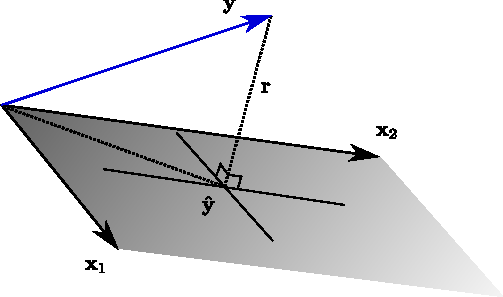
\includegraphics[width=0.5\textwidth]{residu_orth}%
%         \caption{Second example}
%         \label{subfig:logo}
%     \end{subfigure}
%     \caption{Exemples of side by side images}
%     \label{fig:double_example}
% \end{figure}

Magneto-/electroencephalography (M/EEG) allows for a non-invasive analysis of
functional brain imaging (\cite{Baillet_Mosher_Leahy_2001}). The distributed-source approach models the brain activity
with a fixed number of dipoles distributed over a dense three-dimensional 
grid within the brain volume (\cite{Dale_Sereno_1993}). The task in the inverse problem is to estimate the 
distribution of dipolar currents over this three-dimensional grid that can explain the 
measured data. Since the number of dipoles is typically much larger than the number 
of sensors placed on the scalp of the subject, source localization is an 
ill-posed inverse problem having an infinite number of solutions. In order to render
the solution unique, biologically-plausible constraints must be applied on the optimization
problem. Literature is awash of inverse methods favoring sparse solutions to explain the
M/EEG signals including parametric (\cite{Huang_Breheny_Ma_2012}; \cite{Matsuura_Okabe_1995}; 
\cite{Uutela_Hamalainen_Somersalo_1999}) and Bayesian approaches (\cite{Costa_Batatia_Oberlin_DGiano_Tourneret_2017}; 
\cite{Oikonomou_Kompatsiaris_2020}). Those techniques are suitable for short-term source reconstruction 
- typically for tens of milliseconds after the cognitive stimulus - but fails for larger time frame when the 
stationarity assumption needs to be relaxed (\cite{Gramfort_Strohmeier_Haueisen_Hamalainen_Kowalski13}). 
In recent years, a promising approach has been Mixed Norm Estimate (MxNE) 
(\cite{Gramfort_Kowalski_Hamalainen12}), that extends the Lasso (\cite{Tibshirani96}), 
a regularized least-square model that applies a $\ell_1$-norm penalty on the coefficients to yield 
sparse solutions. More precisely, MxNE is a multi-task Lasso
model that imposes a block separable convex penalty with a $\ell_{2,1}$-mixed-norm, similar to 
Group Lasso (\cite{Yuan_Lin06}) or Group Basis Pursuit (\cite{Liao_Li_Carin_2014}). We refer to 
\cite{Bach_Jenatton_Mairal_Obozinski12} for a comprehensive review of sparsity-inducing norms. 
Each block represents the source activation over time of a dipole with fixed or free orientation at a specific source location.
\cite{Strohmeier_Bekhti_Haueisen_Gramfort_2016} improved MxNE by proposing iteratively reweighted Mixed Norm Estimate 
(irMxNE), a M/EEG sparse source imaging approach based on the iterative reweighting of the $\ell_1$-
norm (\cite{Candes_Wakin_Boyd08}).

All those approaches are parametrized by one hyperparameter that controls the sparsity level
induced by the constraint. Figure 1 shows the critical effect of this regularizing hyperparameter 
on the sparsity of the solution. The larger the hyperparameter, the sparser the solution which translates
into fewer sources recovered by the model. Hyperparameter selection remains a challenging yet crucial task
for inverse problems. Various approaches have been proposed to automatically select the regularizing 
hyperparameter in sparse models. Bayesian approaches consist in setting a prior distribution 
and select the hyperparameter by \textit{maximum-a-posteriori} (MAP) estimation (\cite{Pereyra_BioucasDias_Figueiredo_2015};
\cite{Vidal_Bortoli_Pereyra_Durmus_2020}; \cite{Hashemi_Cai_Kutyniok_Muller_2020}).
\cite{Pereyra_BioucasDias_Figueiredo_2015} introduced two hierarchical Bayesian methods to perform MAP 
inference when the value of the regularization parameter is unknown, by setting a Gamma prior on the 
unknown hyperparameter. \cite{Bekhti_Badeau_Gramfort_2017} adapted this method to the multi-task Lasso problem
for source localization and proposed a method to adjust the scale parameters $\alpha$ and $\beta$
of the Gamma prior. However, both methods require to fine-tune at least one parameter by hand, which is a
tedious process for non-experts. Hyperparameter selection can also be done using an exhausive
grid-search using a held-out criterion (\cite{Bergstra_Bengio12}, \cite{BergstraBardenetBengioKegl2011}): 
the model is fitted for a range of possible values of the hyperparameter, which are fixed within each individual optimization. 
The hyperparameter that maximizes some criterion is then used as an unbiased estimate of the true hyperparameter value.
\cite{Pedregosa16} has showed that cross-validating the hyperparameter on held-out sets is not a suitable approach for inverse 
problems. Figure 2 shows that cross-validation (CV) consistently performs worse than other 
hyperparameter selection methods. CV requires the i.i.d. assumption to be fulfilled, which is 
not the case when dealing with an array of spatially-correlated sensors. The crucial question revolves around
finding a good estimator of the reconstruction error of a model. \cite{Stein81} proposed an unbiased estimator
of the quadratic risk of models, called Stein's Unbiased Risk Estimator (SURE). SURE has proved to be 
useful for digital signal and image reconstruction (\cite{Pesquet_Benazza_Chaux_2009}) and for
parameter selection (\cite{Deledalle_Vaiter_Fadili_Peyre14}). 
\\
In this paper, we introduce a procedure based on the Monte-Carlo finite difference SURE 
(\cite{Deledalle_Vaiter_Fadili_Peyre14}; \cite{Ramani_Blu_Unser08}) that achieves state-of-the-art performance on hyperparameter 
selection tasks for MxNE and irMxNE. The three main contributions of this article are as follows:

\begin{enumerate}
    \item We derive a closed-form formulation of SURE for MxNE and show how to evaluate SURE numerically
    for irMxNE.

    \item We propose one algorithm based on SURE to automatically select regularizing hyperparameter for irMxNE
    in the context of the M/EEG source localization problem.

    \item We show that our hyperparameter selection technique for irMxNE achieves state-of-the-art results on real M/EEG data.
\end{enumerate}

An implementation of our code can be found in MNE software (\cite{mne}).
The different strategies are tested on simulations and multiple source reconstruction 
problems using public M/EEG data.
%
\newline
\newline
%
\textit{\textbf{Notation}} The transpose of a matrix $\mathbf{A} \in \mathbb{R}^{M \times N}$ is
denoted $\bf{A}^\top$. $\mathbf{A}_{i:}$ and $\mathbf{A}_{:j}$ correspond to the $i^{th}$
row and the $j^{th}$ column respectively. $\norm{A}_{\text{F}}$ indicates the Frobenius norm,
and $\norm{\mathbf{A}}_{p,q}$ the $\ell_{p,q}$-mixed-norm with $\norm{\mathbf{A}}_{p,q} 
= \left(\sum_i \left(\sum_j \lvert \mathbf{A}[i,j] \rvert^p\right)^{q/p}\right)^{1/q}$.
$\mathbf{I}$ denotes the identity matrix.


%%%%%%%%%%%%%%%%%%%%%%%%%%%%%%%%%%%%%%%%%%%%%%%%%%%%%%%%%%%%%%%%%%%%%%%%%%%%%%%
\subsection{Background}
\label{sub:background}
%%%%%%%%%%%%%%%%%%%%%%%%%%%%%%%%%%%%%%%%%%%%%%%%%%%%%%%%%%%%%%%%%%%%%%%%%%%%%%%
%

\subsubsection{The Mixed Norm estimate (MxNE) and its reweighted formulation}

The M/EEG source localization problem can be described by the linear forward model:

\begin{equation} \label{eq:1}
    \mathbf{M = GX + E}
\end{equation}
%
where $\mathbf{M} \in \mathbb{R}^{N \times T}$ is a measurement matrix where $N$ is the
number of sensors placed on the scalp and $T$ is the number of time instants of the measurements.
$\mathbf{G} \in \mathbb{R}^{N \times S}$ is the design matrix, a known 
instantaneous mixing matrix also called the gain matrix and $S$ is the number of source locations.
This matrix relates the source
to the measurements. $\mathbf{E} \in \mathbb{R}^{N \times T}$ is the noise matrix, which
is assumed to be additive, white and Gaussian, $\mathbf{E}[:,j] \sim \mathcal{N}(0, \mathbf{I})
\enspace \forall j$. $\mathbf{X} \in \mathbf{R}^{S \times T}$ is the coefficient matrix to be estimated. 
It corresponds at every point in time to the estimated current intensity at the dipoles in
the brain volumes. This model can be further extended considering multiple degrees of freedom of the current dipole
per source location. $\mathbf{X}$ can be partitioned into $S$ blocks $\mathbf{X}_s \in \mathbb{R}^{O \times T}$, where
each $\mathbf{X}_s$ represents the source activation at a specific source location $s$ and $O$ is the number of 
degrees of freedom. In the rest of the paper, we shall refer as fixed orientation when $O = 1$ and
free orientation when $O = 3$. Assuming a known regularization parameter $\lambda > 0$, we recall the multi-task
Lasso regression model defined by:

\begin{equation} \label{eq:2}
    \widehat{\mathbf{X}} \in \argmin_{\mathbf{X}}
    \frac{1}{2}\norm{\mathbf{M - GX}}^2_{\text{F}}
    + \lambda \mathcal{P}(\mathbf{X})
    \enspace ,
\end{equation}
%
where $\mathcal{P}(\mathbf{X})$ is a regularization term and $\lambda \in \mathbb{R}$ the hyperparameter
that controls the trade-off between the data-fit and the penalization. \cite{Gramfort_Kowalski_Hamalainen12}
introduced MxNE where $\mathcal{P}(\mathbf{X}) = \norm{\mathbf{X}}_{2, 1}$ to promote spatially focal sources with
smooth temporal estimates:

\begin{align} \label{eq:3}
    \widehat{\mathbf{X}} 
    &\in
    \argmin_{\mathbf{X}}
    \frac{1}{2}\norm{\mathbf{M - GX}}^2_{\text{F}}
    + \lambda  
    \underbrace{\sum_{i=1}^{S} \norm{\mathbf{X}_{i:}}_{2}}_{\triangleq \norm{\mathbf{X}}_{2, 1}}
    \enspace .
\end{align}
%
MxNE is a convex optimization problem that can be solved using proximal gradient descent (\cite{Nesterov05}; \cite{Nesterov09}; \cite{Beck_Teboulle09})
or block coordinate descent (\cite{Tseng_Yun09}; \cite{Wright2015}; \cite{Massias_Vaiter_Gramfort_Salmon20}). \cite{Strohmeier_Bekhti_Haueisen_Gramfort_2016} built upon MxNE to propose the iterative reweighted MxNE (irMxNE) optmization
scheme:

\begin{equation} \label{eq:5}
    \widehat{\mathbf{X}}^{(k)}
    \in
    \argmin_{\mathbf{X}}
    \frac{1}{2}\norm{\mathbf{M - GX}}^2_{\text{F}}
    + \lambda \sum_{i=1}^{S} 
    \frac{\norm{\mathbf{X}_{i:}}_2}
    {2 \sqrt{\norm{\widehat{\mathbf{X}}^{(k-1)}_{i:}}_2}}
    \enspace .
\end{equation}
%
irMxNE consists in minimizing a concave objective by iteratively solving convex surrogate problems. Therefore, we are not guaranteed to
converge to a global minimum, the results depend on the initialization of the weights used. As a rule of thumb, \cite{Candes_Wakin_Boyd08} argues
that the weights should relate inversely to the true signal magnitude. \cite{Strohmeier_Bekhti_Haueisen_Gramfort_2016} proposed to initialize
the weights at 1, which is tantamount at the first iteration to solve a standard MxNE problem.

\subsubsection{Stein's unbiased risk estimate (SURE) for MxNE}

We now explain how to automatically select $\lambda \in \mathbb{R}$ in MxNE. Considering, the solution of 
\eqref{eq:3} $\widehat{\mathbf{X}}$ and the unknown true parameter $\mathbf{X}^*$, the quadratic risk of $\widehat{\mathbf{X}}$
reads:

\begin{equation} \label{eq:6}
    \text{MSE}(\widehat{\mathbf{X}})
    = \mathbb{E}_{\mathbf{E}}
    \left[
        \norm{
            \mathbf{X}^* - \widehat{\mathbf{X}}
        }_{\text{F}}^2
    \right]
    \enspace .
\end{equation}
%
Since MSE is unknown, \cite{Stein81} proposed an unbiased estimator of $\text{MSE}(\widehat{\mathbf{X}})$,
which writes:

\begin{align} \label{eq:7}
    \text{SURE}(\widehat{\mathbf{X}})
    &= -nT\sigma^2 + \norm{
        \mathbf{M} - \mathbf{G}\widehat{\mathbf{X}}
    }_{\text{F}}^2
    + 2 \sigma^2 \text{df}(\widehat{\mathbf{X}})
    \enspace ,
\end{align}
%
where $\text{df}(\widehat{\mathbf{X}})$ is the number of degrees of freedom of $\widehat{\mathbf{X}}$,
alternatively called the divergence of $\widehat{\mathbf{X}}$ and $\sigma^2$ is the noise variance of the measurements. 
SURE is an estimator of $\text{MSE}$ that needs to verify some non-trivial assumptions, 
the most notable of which being that the estimator must be weakly differentiable with respect to $\mathbf{M}$. 
A detailed proof of this assumption can be found in \cite{Zou_Hastie_Tibshirani07}
for LASSO-like models. As argued by \cite{Deledalle_Vaiter_Fadili_Peyre14}, the standard approach to evaluate the divergence
of an estimator is to exploit the fact that the divergence only depends on the trace of $\mathcal{J}_{\widehat{\mathbf{X}}}(\mathbf{M})$,
where $\mathcal{J}_{\widehat{\mathbf{X}}}(\mathbf{M})$ is the Jacobian of the mapping $\mathbf{M} \rightarrow \widehat{\mathbf{X}}(\mathbf{M})$.
\\
\\
In the following, we derive the closed-form divergence of SURE for MxNE. Let $A$ be the active set 
of the MxNE and $\mathbf{S}_A$ a matrix filled at every time instant with the signs of the coefficients of the active set. 
Besides, we denote by $\mathbf{G}_A$ (respectively $\mathbf{X}_A$) the restriction of $\mathbf{G}$ (respectively $\mathbf{X}$) to its activated
columns (respectively rows). Finally, let $\mathbf{\Lambda} = \text{diag}(\lambda)$.
To derive a closed-form solution of SURE for MxNE, we make the reasonable assumption that the active set $A$ and $\mathbf{S}_A$ are locally constant, 
meaning that a small change in $\mathbf{M}$ does not change the active set nor the signs of the active 
coefficients. First, let's examine the multi-task LASSO fit column-wise (\textit{i.e.} task by task), for 
$t = 1, \dots, T$:

\begin{equation*}
    \mathbf{G\widehat{X}}_{:t}
    = \mathbf{G}_A (\mathbf{G}_A^{\top}\mathbf{G}_A)^{-1}
    \left(
        \mathbf{G}^{\top}_{A}\mathbf{M}_{:t}
        -
        \mathbf{\Lambda} (\mathbf{S}_{A})_{:t}
    \right)
\end{equation*}
%
The degrees of freedom of MxNE writes:

\begin{align*}
    \text{df}(\widehat{\mathbf{X}}) 
    &= \sum_{i=1}^n \sum_{t=1}^T
    \frac{
        \partial (\mathbf{G}\widehat{\mathbf{X}})_{i, t}
    }{
        \partial (\mathbf{M})_{i, t}
    } \\
    &= \sum_{t=1}^T \left(
        \sum_{i=1}^n \frac{
            \partial (\mathbf{G}\widehat{\mathbf{X}})_{i, t}
            }{
                \partial (\mathbf{M})_{i, t}
            } 
    \right) \\
    &= \sum_{t=1}^T \text{tr}(
        \mathbf{G}_A (\mathbf{G}_A^{\top}\mathbf{G}_A)^{-1}\mathbf{G}_A^{\top}
    ) \\
    &= T \lvert A \rvert
    \enspace ,
\end{align*}
%
which gives the closed-form divergence of SURE for MxNE:

\begin{equation} \label{eq:8}
    \text{SURE}(\widehat{\mathbf{X}})
    = -nT\sigma^2 + \norm{
        \mathbf{M} - \mathbf{G}\widehat{\mathbf{X}}
    }_{\text{F}}^2
    + 2 \sigma^2 T \lvert A \rvert
    \enspace .
\end{equation}

\subsubsection{Evaluating SURE for irMxNE}

The non-convex penalty used at \eqref{eq:5} prevents the derivation of a general closed-form solution for SURE and would make 
the evaluation of the divergence term very costly. In the following, 
SURE is evaluated numerically using a combination of Monte-Carlo sampling technique and finite difference method. 
We insist on the power of this approach as it is a black-box method which only uses the output of the estimator without neeeding
any information on its functional form, making it applicable to a wide range of estimators.
A comprehensive review of techniques to evaluate SURE can be found in \cite{Deledalle_Vaiter_Fadili_Peyre14}.
The Monte-Carlo sampling technique consists in evaluating the degrees of freedom by randomly sampling $N$ vectors that will 
serve to compute $N$ directional derivatives of the mapping $\mathbf{M} \rightarrow \widehat{\mathbf{X}}(\mathbf{M})$, where 
$\widehat{\mathbf{X}}$ is an estimator obtained with irMxNE. More formally, \cite{Deledalle_Vaiter_Fadili_Peyre14} infers that:

\begin{equation} \label{eq:9}
    \text{df}(\widehat{\mathbf{X}}) = 
    \sum_{t=1}^T
    \mathbb{E}_{\Delta_t \sim \mathcal{N}(0, \mathbf{I}_N)}
    \left\langle
        \frac{
            \partial \widehat{\mathbf{X}}_{:t}
        }{
            \partial \mathbf{M}_{:t}
        }[\Delta_t],
        \mathbf{G}\Delta_t
    \right\rangle
\end{equation}
%
where $\frac{\partial \widehat{\mathbf{X}}_{:t}}{\partial \mathbf{M}_{:t}}[\Delta_t]$ is the directional derivative of $\widehat{\mathbf{X}}$ w.r.t.
$\mathbf{M}$ in the direction of $\Delta_t$.
We observe numerically that for the recovery problems we consider, it provides an accurate estimator of the trace, while it only
costs in the multi-task case $\mathcal{O}(TN)$. Now, we need to efficiently evaluate the directional derivative 
$\frac{\partial \widehat{\mathbf{X}}_{:t}}{\partial \mathbf{M}_{:t}}[\Delta_t]$, for $t=1,\dots, T$. A finite difference method reads:

\begin{equation} \label{eq:10}
    \frac{\partial \widehat{\mathbf{X}}_{:t}}{\partial \mathbf{M}_{:t}} 
    [\Delta_t]
    = \lim_{\epsilon \rightarrow 0}
    \frac{
        \widehat{\mathbf{X}}_{:t}(\mathbf{M}_{:t} + \epsilon \Delta_t)
        -
        \widehat{\mathbf{X}}_{:t}(\mathbf{M}_{:t})
    }{\epsilon}
    \enspace .
\end{equation}
%
This generic method allows us to circument the hurdle of evaluating a closed-form expression for each penalty
in the case of irMxNE. \cite{Deledalle_Vaiter_Fadili_Peyre14} observes that in practice this method yields a 
quasi-unbiased risk estimator and found a heuristic for $\epsilon = 2\sigma / n^{0.3}$. Finally combining equations
\eqref{eq:9} and \eqref{eq:10}, Finite Difference Monte Carlo (FDMC) SURE applied to irMxNE writes:

\begin{equation} \label{eq:11}
    \text{df}(\widehat{\mathbf{X}}) = 
    \lim_{\epsilon \rightarrow 0}
    \frac{1}{\epsilon}
    \sum_{t=1}^T
    \mathbb{E}_{\Delta_t \sim \mathcal{N}(0, \mathbf{I}_N)}
    \left\langle
        \widehat{\mathbf{X}}_{:t}(\mathbf{M}_{:t} + \epsilon \Delta_t)
        -
        \widehat{\mathbf{X}}_{:t}(\mathbf{M}_{:t})
        ,
        \mathbf{G}\Delta_t
    \right\rangle
\end{equation}
%
\underline{Proof}: We will prove the previous equality for $t=1, \dots, T$. Let
$\epsilon > 0$ and $\Delta_t$ be a zero-mean i.i.d. random vector independent of
$\mathbf{M}_{:t}$ with unit variance and bounded higher moments.
\\
\\
Writing the second-order Taylor expansion of $\widehat{\mathbf{X}}_{:t}(\mathbf{M}_{:t})$,

\begin{equation*}
    \widehat{\mathbf{X}}_{:t}(\mathbf{M}_{:t} + \epsilon \Delta_t) =
    \widehat{\mathbf{X}}_{:t}(\mathbf{M}_{:t})
    + \epsilon \mathcal{J}_{\hat{\mathbf{X}}_{:t}}(\mathbf{M}_{:t}) \Delta_t
    + \epsilon^2 r_t
    \enspace .
\end{equation*}
%
where $\mathcal{J}_{\widehat{\mathbf{X}}_{:t}}(\mathbf{M}_{:t})$ is the Jacobian of $\widehat{\mathbf{X}}_{:t}$
evaluated at $\mathbf{M}_{:t}$ and $r_t$ is a residual term that tends towards 0 when $\epsilon$ is infinitely
small. It follows that:

\begin{equation*}
    \frac{1}{\epsilon}
        \left(
            \Delta_t^{\top} (\widehat{\mathbf{X}}_{:t}(\mathbf{M}_{:t}
            + \epsilon \Delta_t) - \widehat{\mathbf{X}}_{:t}(\mathbf{M}_{:t}))
        \right)
    =
    \Delta_t^{\top} \mathcal{J}_{\widehat{\mathbf{X}}_{:t}}(\mathbf{M}_{:t}) \Delta_t
    + \epsilon \Delta_t^{\top}r_t
\end{equation*}
%
Taking the expectation on both sides, it follows:

\begin{align*}
    \mathbb{E} \left(
        \frac{1}{\epsilon}
        \left(
            \Delta_t^{\top} (\widehat{\mathbf{X}}_{:t}(\mathbf{M}_{:t}
            + \epsilon \Delta_t) - \widehat{\mathbf{X}}_{:t}(\mathbf{M}_{:t}))
        \right)
    \right)
    &=
    \mathbb{E} \left(
        \Delta_t^{\top} \mathcal{J}_{\widehat{\mathbf{X}}_{:t}}(\mathbf{M}_{:t}) \Delta_t
    \right) + \epsilon \mathbb{E} \left( \Delta_t^{\top} r_t \right)\\
    &=
    \mathbb{E} \left(
        \tr \left(
            \Delta_t^{\top} \mathcal{J}_{\widehat{\mathbf{X}}_{:t}}(\mathbf{M}_{:t}) \Delta_t
        \right)
    \right) + \epsilon \mathbb{E} \left( \Delta_t^{\top} r_t \right)\\
    &=
    \mathbb{E} \left(
        \tr \left(
            \Delta_t \Delta_t^{\top} \mathcal{J}_{\widehat{\mathbf{X}}_{:t}}(\mathbf{M}_{:t})
        \right)
    \right) + \epsilon \mathbb{E} \left( \Delta_t^{\top} r_t \right)\\
    &=
    \tr \left(
        \mathbb{E} \left(
            \Delta_t \Delta_t^{\top}
        \right)
        \mathcal{J}_{\widehat{\mathbf{X}}_{:t}}(\mathbf{M}_{:t})
    \right) + \epsilon \mathbb{E} \left( \Delta_t^{\top} r_t \right)\\
    &=
    \tr \left(
        \mathcal{J}_{\widehat{\mathbf{X}}_{:t}}(\mathbf{M}_{:t})
    \right) + \epsilon \mathbb{E} \left( \Delta_t^{\top} r_t \right)
\end{align*}
%
Therefore,

\begin{equation*}
    \lim_{\epsilon \rightarrow 0} \mathbb{E} \left(
        \frac{1}{\epsilon}
        \left(
            \Delta_t^{\top} (\widehat{\mathbf{X}}_{:t}(\mathbf{M}_{:t}
            + \epsilon \Delta_t) - \widehat{\mathbf{X}}_{:t}(\mathbf{M}_{:t}))
        \right)
    \right)
    = \tr \left(
        \mathcal{J}_{\widehat{\mathbf{X}}_{:t}}(\mathbf{M}_{:t})
    \right)
\end{equation*}
%


Based on this method of evaluating SURE, we propose the following algorithm to automatically select $\lambda \in \mathbb{R}$ for irMxNE.

\vskip 0.2in

{\fontsize{4}{4}\selectfont
\begin{algorithm}[h]  % again h stands for here
\SetKwInOut{Input}{input}
\SetKwInOut{Init}{init}
\SetKwInOut{Parameter}{param}
\caption{\textsc{Automatic hyperparameter selection for irMxNE with SURE MCFD}
}
%
\Input{$
    \mathbf{G} \in \bbR^{N \times S},
    \mathbf{M} \in \bbR^{N\times T},
    \lambda_{\text{max}} \in \bbR^+_,
    \lambda_{\text{min}} \in \bbR^+_,
    $}
    \Init{$
    \text{SURE}_{\text{best}} = \infty,
    \lambda_{\text{best}} = \lambda_{\text{max}},
    \Delta_t \sim \mathcal{N}(0, \mathbf{I}_N),
    \epsilon > 0
    $}

    \For{$\lambda = \lambda_{\text{max}},\dots, \lambda_{\text{min}}$}
    {
        Solve irMxNE minimization problem for $\lambda$:
        $\widehat{\mathbf{X}} \leftarrow \text{irMxNE}(\mathbf{G}, \mathbf{M}, \lambda)$

        Compute divergence of SURE with \eqref{eq:11}

        Compute SURE with \eqref{eq:7}

        If $\text{SURE} \leq \text{SURE}_{\text{best}}$:
        $\text{SURE}_{\text{best}} \leftarrow \text{SURE}$
        $\lambda_{\text{best}} \leftarrow \lambda$
    }

\Return{$\mathbf{B}$}
\end{algorithm}
}

\subsubsection{Reformulation of SURE in the time-frequency domain}


%%%%%%%%%%%%%%%%%%%%%%%%%%%%%%%%%%%%%%%%%%%%%%%%%%%%%%%%%%%%%%%%%%%%%%%%%%%%%%%
\subsection{Experience}
\label{sub:experience}
%%%%%%%%%%%%%%%%%%%%%%%%%%%%%%%%%%%%%%%%%%%%%%%%%%%%%%%%%%%%%%%%%%%%%%%%%%%%%%%
%

%%%%%%%%%%%%%%%%%%%%%%%%%%%%%%%%%%%%%%%%%%%%%%%%%%%%%%%%%%%%%%%%%%%%%%%%%%%%%%%
\subsection{Implementation details}
\label{sub:experience}
%%%%%%%%%%%%%%%%%%%%%%%%%%%%%%%%%%%%%%%%%%%%%%%%%%%%%%%%%%%%%%%%%%%%%%%%%%%%%%%
%
Free fixed solver
Warm start

\clearpage
